\section*{Неразмеченные данные в глубоком обучении}

\section{Постановка}
\hspace{2em}Общий подход к решению задачи с неразмеченными данными следующий:

$\mathcal{U} \subset \mathcal{X}$ --- большая неразмеченная выборка,

$\mathcal{D} \subset  \mathcal{X}\times \mathcal{Y}$ --- небольшая размеченная выборка,

требуется построить отображение $f: \mathcal{X} \to \mathcal{Y}$.

\section{Суперпозиция}
\hspace{2em}Предположение $f = c  \circ  h$ --- отображение есть суперпозия двух функций:

$h$ --- генерация признакового описания $h: \mathcal{X} \to \mathcal{H}$,

$c$ --- классификатор $c: \mathcal{H} \to \mathcal{Y}$.

Заметим, что $c$ и $h$, например, это некоторое параметрические функции, параметры которых нужно найти.

Простой пример:

$h$ --- все слои полносвязного многослойного перцептрона,

$c$ --- последний слой.

Обычно $h$ является сложной моделью, а $c$ --- линейной. Рассмотрим более подробный пример.

\section{Постановка задачи SimCLR}

\hspace{2em}Постановка задачи SimCLR заключается в том, что даётся набор изображений без каких-либо меток, и нужно обучить модель на этих данных так, чтобы она могла быстро адаптироваться к любой задаче распознавания изображений впоследствии.

Цель обучения - найти такое признаковое пространство, в котором изображения одного класса располагаются близко по введённой метрике, а изображения разных классов - далеко. Для этого используют различные \textit{контрастивные функции потерь}.

\begin{figure}
    \centering
    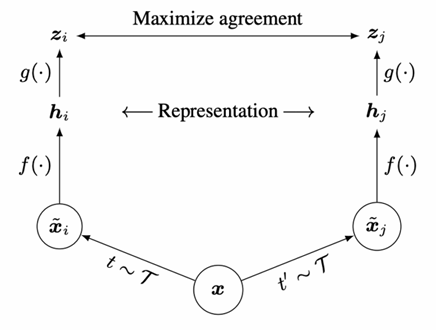
\includegraphics[width=0.5\linewidth]{simclr.png}
    \caption{Схематичное представление алгоритма SimCLR}
    \label{fig:enter-label}
\end{figure}

На рисунке можем схематичное представление последовательности шагов алгоритма со следующими обозначениями:

\begin{quote}
$x$ - исходное изображение,

$t, t'$ - разные аугментации на исходное изображение $x$ для получения представлений $\tilde{x_i}$, $\tilde{x_j}$,

$f$ - функция, генерирующая представления (representation) $h_i$, $h_j$ в виде вектора для входных изображений,

$g$ - функция, которая переводит вектора $h_i$, $h_j$ в величины $z_i$, $z_j$, для которых минимизируется расстояние (maximize agreement) в процессе обучения для аугментаций одного изображения и максимизируется для разных изображений.
\end{quote}

Шаги в обучении следующие:

1. К исходному изображению $x$ применяются аугментации $t, t'$. \textit{Аугментация} - это процесс создания новых данных на основе существующих с помощью преобразований. Такими преобразованиями для изображений являются, например, поворот, изменение яркости, гауссовское размытие и так далее. Она необходима, чтобы в новом признаковом пространстве изменённые изображения так же находились близко к изображениям того же класса.

2. К аугментированным изображениям $\tilde{x_i}$, $\tilde{x_j}$ применяется функция $f$, генерирующая векторное представление этих изображений $h_i$, $h_j$.

3. К векторным представлениям $h_i$, $h_j$ применяется функция $g$ для перевода в другое векторное представление. Данный шаг необязательный для обучения методом SimCLR.

4. Для $z_i$, $z_j$ уменьшается расстояние, если $\tilde{x_i}$, $\tilde{x_j}$ - аугментации одного и того же изображения, и увеличивается - если разных. Происходит это путём минимизации контрастивной функции потерь. 

Таким образом мы находим новое признаковое описание для изображения, с помощью которого можно обучиться на задачу классификации изображений, то есть найти функция $c$ из раздела про Суперпозицию.

\section{Вопросы}
\hspace{2em}1. Что такое суперпозиция в контексте построения модели для неразмеченных данных, и как она помогает в решении задачи с использованием методов глубокого обучения?

2. Каковы основные этапы и задачи в методе SimCLR?

3. Как аугментация данных способствует улучшению качества обучаемых представлений?
